% preliminaries %
\documentclass[11pt,letterpaper,onecolumn,twoside,openright,draft]{report}

\usepackage{graphicx}
%\usepackage[dvips,bookmarks,colorlinks=false,pdfkeywords={PDF, LaTeX, hyperlinks, hyperref}]{hyperref}
\usepackage[bookmarks,colorlinks=false,pdfkeywords={PDF, LaTeX, hyperlinks, hyperref}]{hyperref}
\hypersetup{backref,pdfpagemode=FullScreen,colorlinks=true}
\usepackage{todonotes}

% front matter %
\begin{document}
\title{Routes: A Multiagent Taxi Simulation}
\author{Tim Condit}
\date{\today}
\maketitle
\thispagestyle{empty}

\hyphenation{a-gents au-ton-o-mous great-er mul-ti-a-gent pa-ra-digms slight-ly}

% use roman numerals for the front matter %
\pagestyle{headings}
\setcounter{page}{1}
\pagenumbering{roman}

\tableofcontents
\todo{add hyperlinks}
\listoffigures
\listoftables

% Break lines at sentences for version control sake.  Good stuff here:
% http://stackoverflow.com/questions/193298/best-practices-in-latex/196724#196724

% abstract (no page number) %
\begin{abstract}
Routes is a multiagent simulation of a Taxi service and its Fares.
All Taxis are created at the beginning of the simulation.
While the program is running, Fares enter the system at random times in random places.
Rather than requesting pickup through a central dispatch, the Fares broadcast their own locations locally, then regionally, and finally throughout the entire area, if needed.
Starting with the local region, all Taxis in a given range receive the Fare's pickup request and may decide to act on it, or they may ignore it, depending on their circumstances and the type of simulation being run.

Functional transit maps are generated in real-time from Census Bureau data that includes the entire United States of America and territories.
The size of the transit map, and hence the simulation's range can be as small as a single area code, up to an entire county.
The data that is downloaded to generate the transit map is processed locally the first time it's used, and cached to save time (and bandwidth) for subsequent runs.

\todo{Add something here about the transit map being a big network graph. Can probably pull something directly out of the full text.}

There are three different negotiation protocols - first-in, first-out, closest Fare, and mixed mode.
There are two simulation types - cooperative and competitive.
They are combined for a total of six different simulations.
\end{abstract}

% switch to Arabic numbers for the body - and restart the page count %
\pagenumbering{arabic}
\setcounter{page}{2}

% introduction %
\chapter{Introduction}

Routes is a simulation of a taxi service.

Taxi services have operated the same way for many years.
Wherever they operate, it is common to get a ride by flagging down a taxi from the side of the road.
Most taxi companies also have dispatchers who will arrange pickup at a later time.
\footnote{A notable exception is New York City, where a fare cannot be prearranged.
Only for-hire vehicles such as livery cars or limousines may prearrange pickup.

{\hyperlink{http://www.nyc.gov/html/tlc/downloads/pdf/fhv_base_fact_sheet.pdf}{Understanding the For-Hire Vehicle Industry}}
\hyperlink{http://www.nyc.gov/html/tlc/html/passenger/faq_pass.shtml\#14} {How can I pre-arrange a trip in a Yellow Cab?}}

\todo{the hyperlinks below are broken}

Taxi services are subject to extensive regulation, and are in some ways similar to a public utility.

\footnote{This site documents legal actions and taxi regulations all over the world: {\hyperlink{http://www.taxi-library.org/regulation.htm}{Regulation of Taxicabs}}}

For example, the rates charged by municipal taxi services are often set by the city or county in which the taxis operate.
This means that among other things, they cannot compete on price, since they are all forced to charge the same rates for the same trips.

The simulations presented in this paper have none of these restrictions.
They are closer to a loose confederation of independent drivers than to a highly regulated municipal utility.
They are missing a couple key features of terrestrial taxis.
First, they cannot be flagged down for a pickup.
If they are not on their way to pick up a Fare, or driving the Fare to it's destination, they are not moving.
Second, they do not have a dispatcher.
This is a key component.
They operate in a distributed fashion, with the Fare initiating contact with the Taxis directly, and - in the cooperative simulations anyway - the Taxis communicating amongst themselves about which one will pick up a given Fare.

They ask and try to answer the following questions:
\begin{itemize}
  \item{Is an autonomous, distributed Taxi system technically feasible, at least conceptually?
    How would it work?}
  \item{How would the dynamic change when Agents (Fares and Taxis) communicate with each other directly?}
  \item{Would a Fare be willing to wait a little longer for a better price?
    (This implies that the now hidden cost of driving to a Fare is explicitly included in the cost of the fare, since without the cost of making the pickup there is no chance to earn the revenue of the trip.)}
  \item{What would happen if both the Taxi and the Fare had to be satisfied that the trip was worthwhile?
    And what if as a result of these constraints, some Fares get no service?}
  \item{What would happen if Taxis had to compete for Fares with their fellows?
    Would this improve service for all?
    Or would a cooperative model work better at the team or organization level?}
  \item{What would happen if two teams of Taxis competed with each other?
    In other words, the Taxis of two teams A and B would coordinate Fare pickup amongst themselves, but they’d be competing with the other team, and will lose some of the Fares.
    Would the results be much different at the system level than what happens when it’s "every man for himself"?}
\end{itemize}

But mostly this is a paper that explores the use of autonomous agents.
They are characterized this way in \cite{roozemond2000act}, in a section called "What are intelligent agents?":

\quote{Multi-Agent Systems can be characterised by the interaction of many agents trying to solve a variety of problems in a cooperative fashion.
Besides AI, intelligent agents should have some additional attributes to solve problems by itself in real-time; understand information; have goals and intentions; draw distinctions between situations; generalise; synthesise new concepts and/or ideas; model the world they operate in and plan and predict consequences of actions and evaluate alternatives.
The problem solving component of an intelligent agent can be a rule-based system but can also be a neural network or a fuzzy expert system.}

The Agents in this series of simulations meet most of these criteria.
In half the simulations the Agents work together in a cooperative fashion - in the other half, they are competitive; they are able to solve problems by themselves in real-time; they understand Fare requests for pickup (information); they have goals and intentions; and they draw distinctions between situations to determine whether to reserve (or compete for) a particular Fare.
They don't do much generalizing or synthesizing of new concepts, but they do model the world in which they operate, and predict the consequences of their actions and act accordingly.

The Agents are Taxis and Fares, but in another context they may have been viruses and antibodies, or cowboys and indians.
Both may draw attention away from the simulations, in different directions: viruses and antibodies may be too complex, and cowboys and indians may be too simple.
Taxi services in the real world do not have many competitive freedoms.
The main goal of all the regulation seems to be about providing a reliable service with predictable prices.
Those are fine goals, but the simulations in this paper step outside those boundaries, and explore what would happen if things were allowed to evolve differently.

The higher priority for this paper was flexibility in designing the negotiation protocols and simulations.
Taxis and Fares are not the only choice of autonomous agents to study, but they serve the purpose well.
% that last bit sounds like it belongs in the conclusion

\section{Definition of Terms}
The following terms are used throughout the paper:
\todo{add the definitions!}

\section{Organization}
The rest of the paper consists of the following sections:

\begin{itemize}
  \item{RELATED WORK is a review of the literature.
    Research on taxis as autonomous agents is scarce, but there are traffic and road network simulations that come at the issue from a different direction.
    Instead of looking at a system of mobile agents, stationary agents at traffic lights provide information for improving the flow of traffic or routing around accidents and congestion.
    The Belief-Desire-Intention model of intelligent agents is reviewed, and the Routes agents are categorized within a framework for organizing classes of multi-agent systems for transport logistics.
    (This is not directly related, unless people are considered goods to transport, but it clarifies a few things about the agents nevertheless.)}
  \item{IMPLEMENTATION describes the Taxis and Fares in \linebreak greater detail.
    It explains the grids and graphs that make up the Agent's world, and the network traversal algorithms that calculate routes around the different regions.
    It expands on the negotiation protocols and simulation types.
    Finally it describes the simulation software that drives the whole process, the extensive run-time configuration options, and the interactive environment within which the simulations are executed.}
  \item{RESULTS tells the story of the simulations.
    Individual Agents have autonomy during runtime, but from a simulation point of view, the agents are part of larger system.
    Several simulations are run and their data plotted and reported here.}
  \item{CONCLUSION brings things to a close, and enumerates a number of possible future enhancements.
    There are a number of ways this program could be expanded upon, and the source code will be freely available upon acceptance of this report.}
  \item{APPENDIX A: USING TIGER/LINE DATA describes how raw data from the U.S. Census Bureau, representing roads throughout the United States and it's territories, is converted in real-time into line segments, and how those line segments are knit together to make network graphs upon which the simulations are run.}
  \item{APPENDIX B: ANNOTATED CONFIG FILES enumerates the large collection of both agent and graph data that can be customized at run-time, including full annotations about each setting.}
  \item{APPENDIX C: LIST OF OPEN SOURCE SOFTWARE\ldots}
  \item{APPENDIX D: SOURCE CODE\ldots}
  \item{APPENDIX E: TRANSCRIPT OF INTERACTIVE SESSION\ldots}
\end{itemize}

\todo{existence proof only: get rid of them}
\cite{davidsson2005aab}
\cite{yokoo1999}

% use this?
% cite: http://en.wikipedia.org/wiki/Multi-agent_system, accessed 1/11/2009
%
% Autonomy: the agents are at least partially autonomous
% Local views: no agent has a full global view of the system, or the system is too complex for an agent to make practical use of such knowledge
% Decentralization: there is no one controlling agent (or the system is effectively reduced to a monolithic system)


% related work %
\chapter{RelatedWork}
\section{Introduction}
In this section I examine features found in other multiagent systems to see how they contrast with my system.
The focus in the applied literature is on traffic and road network simulations.
Two of the papers describe centralized versus distributed simulation systems\cite{france2003mso,hernandez2001}.
One of them includes an implemented and installed system, while the other is evaluated using a mathematical formula describing variable levels of traffic congestion.
Aside from the fact that one is applied and the other more theoretical, their approaches are different enough to make a useful comparison.
Then I investigate an uncertainty management framework for understanding relationships between agents in a multiagent sytem\cite{wu2003umf}.
This paper uses the Belief-Desire-Intention (BDI) agent model to formulate a response to received inputs.
The last paper is a review of multi-agent systems (MAS) used for transport logistics\cite{davidsson2005aab}.
My software is classified according to this scheme.

\section{Centralized and distributed multiagent traffic systems}
Reviewing decision support systems (DSS) for use in traffic management.

\subsection{Regional agent coordination with TRYS and TRYSA$_{2}$}
Hern\'{a}ndez et al.\cite{hernandez2001} describes a pair of closely related intelligent traffic management systems (ITMS).
The TRYS\footnote{The acronym is not identified in the paper.} system is implemented and in use in Barcelona, Spain.
TRYSA$_{2}$\footnote{TRYS Autonomous Agents} is developed only to the prototype level at time of publication, but was validated with the same data as the first system.
Both systems partition a highly congested local traffic network into a series of overlapping problem areas, which are monitored by traffic control agents.
These agents collect data via vehicle detectors and telemetered sensors ("loop detectors").
The raw data is used to generate traffic control plans, but they are advisory only.
A human operator makes the final decision on how the plans are used.

These systems are fundamentally different from the approach I have taken for several reasons.
The first, and most important difference is that these are not simulations.
Second, they are open systems in the sense that the outputs are "processed" by a traffic engineer, as opposed to a closed and terminal system, where the final result is the end of the simulation, rather than inputs to an "offline" system.
Finally, the focus here is on the traffic network exclusively, with zero representation of the users of the network, i.e. drivers and passengers.
Regardless, there are some interesting contrasts.

TRYS is a centralized multiagent system.
It operates on inputs from more than 300 telemetered sensors and feed data to the local traffic control center.
The goal of this system is to provide traffic engineers with alternatives for traffic light coordination.
It is more coordinated than autonomous; each agent has to take its neighbor's state into account when designing their traffic control plan.
Imagine a series of traffic lights that are not coordinated with each other in some way.
The individual agents would still generate plans based on the inputs they are receiving.
You might reasonably expect there to be some kind of emergent or spontaneous coordination, but it would most likely not be globally consistent.
Therefore, the local control plans generated by the first-level agents are sent to a special coordinator agent responsible for integrating local control proposals into a coherent global signal plan for the whole traffic network.
The coordinator resolves any conflicts between the local control proposals then sends the globally consistent local signal plans back to the traffic agents.
% and also to the traffic engineer?

An interesting feature of this system is the way in which the agents decide on which traffic control plans to forward to the coordinator.
The agents are provided with data about the traffic congestion ("demand knowledge") and some expectation of how different actions will affect the flow
of traffic ("expected redistribution").
Given these pieces of information, they run a macrosimulation to decide if there will be an adequate decrease in the excess flow.
They forward the plan to the coordinator if appropriate, and reject it otherwise.

TRYSA$_{2}$ is a reformulation of TRYS using autonomous agents.
Whereas TRYS uses a more linear form of communication between the traffic control agents and the coordinator, agents in TRYSA$_{2}$ communicate with one another directly, eliminating the need for a coordinator agent.
See figure~\ref{fig:TRYS-and-TRYSA2} on page~\pageref{fig:TRYS-and-TRYSA2}.

The partitioning of the road network into problem areas is slightly different from that in TRYS, but problem detection, diagnosis and selection of control plans are similar.
Each traffic control agent in TRYSA$_{2}$ maintains its own set of alternative traffic control plans, along with expected reductions in local traffic excesses associated with each of the plans.
This is called the plan's local utility.

This is where things get interesting in TRYSA$_{2}$.
The autonomous agents use a strategy called structural cooperation\cite{ossowski1999}, whereby they take their own utility and the effects of their acquaintances' control plans on their own utiltiy into consideration when deciding what to do.
In short, the agents are no longer fully autonomous.

The paper describes the situation and the response to it this way:

\quote{There is a conflict of interest respecting the way in which local signal plans are adapted.
The essential idea is that the more autonomous an agent is (i.e. the less its local utility can be influenced by others), the more weight will have its opinion respecting which local plans to modify and how to adapt them.
Still, sometimes the resulting basic coordination does not lead to globally optimal control plans, so the system designer can issue rights or prohibitions for some agents to use control devices in certain ways.
By this, he modifies the degree of autonomy of some agents, biasing the outcome of coordination (i.e. the resulting global signal plan) in a desired direction.}

The agents choose local signal plans, but they still need to coordinate with one another to settle on a globally consistent signal plan.
This is similar to the task of the coordinator agent in TRYS.
To do this the agents use a distributed constraint optimization protocol
\footnote{The original basis for my work, although it did not make it into the final product.}
that implements weak commitment search\cite{yokoo1999}.
\todo{This is referenced in Hernandez, but not in this paper.
I should probably dig up the reference anyway.}

This is a three-stage process.
In stage 1 the local control agents repeatedly exchange utility information to find sets of globally compatible alternative signal plans.
Stage 2 starts when one of the agents detects the completion of stage 1.
This agent computes approximate probabilities that each of the chosen sets of local signal plans would be enacted, and from that attempts to maximize the product of the local agent utilities.
In other words, lower quality plans are dropped from consideration.
In stage 3 a set of local signal plans are selected by lottery, and the results are shared with all agents.
This concludes the work of the autonomous agents in TRYSA$_{2}$.
\todo{need something here to break up the flow and signal that we're starting a new section}
At this stage in both systems the selected control plans are ready for review by the traffic engineer.

\subsection{Comparison with Routes}
There are several ways in which these systems differ from mine: they are decision support systems, whereas mine are simulations; they are traffic network-oriented, whereas mine are agent-oriented; one of them is in production use and the other is a prototype, whereas mine is fully implemented but on a smaller scale.
On the other hand, this paper provides something that was hard to come by: a look at similar systems implemented on both a centralized and distributed paradigms.
That and the fact that it was a multiagent traffic management study, made it a useful choice.

One superficial similarity of TRYS and TRYSA$_{2}$ with my system is in the representation of the physical structure of the traffic network.
It uses a declarative description of the network as a graph with nodes and links together with abstraction functions associated to components, described here as "static information about the topological structure of the problem area".
\todo{need something here to break up the flow and signal that we're starting a new section}
Next we look at another multiagent system for optimizing an urban traffic network.

\subsection{Local and Global Agent Coordination}
This paper\cite{france2003mso} is similar in many ways to the previous one.
It is another centralized multiagent system for traffic management that uses local traffic agents and one or more coordinator agents.
But this paper uses traffic intersections as the problem area, rather than larger regions, and builds a hierarchical structure involving other types of coordinating agents as well.

The first goal of this system is to design a traffic network that operates in real-time and takes into account that traffic lights essentially operate in an infinite loop, or as a non-finite process.
The second goal is to handle dynamically occuring events such as traffic accidents or roadway congestion in a coordinated fashion.
With autonomous agents at each intersection, agents at neighboring intersections are unaware of traffic events occuring elsewhere, leading to detrimental traffic flow.
For instance, this system would allow traffic to continue toward a blocked intersection in the case of an accident.
\todo{Does this sentence "With agents at each intersection\ldots" break the flow?}
The final goal is to balance local and global concerns with respect to traffic movement.
Local traffic agents (LTA) will typically have many alternative plans available, but several of them are incompatible with the global goals of traffic management.
A major task is for the coordinator traffic agents (CTA) to quickly figure out which ones to drop from consideration.
This was addressed in Hern\'{a}ndez, but real-time performance data was not provided.

\todo{PICK UP HERE}


\begin{figure}[h]
  %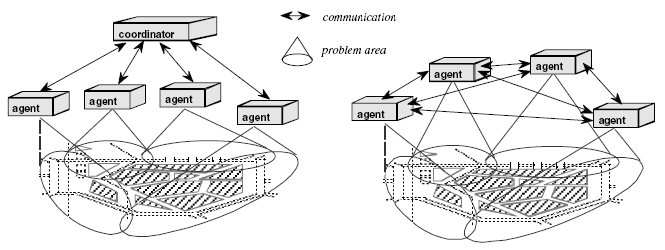
\includegraphics[width=0.8\textwidth]{figures/TRYS-and-TRYSA2.PNG}
  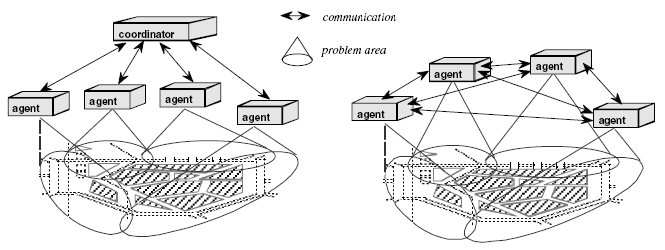
\includegraphics{figures/TRYS-and-TRYSA2.PNG}
  \caption{Centralized (TRYS) and decentralized coordination (TRYSA$_{2}$).}
  \label{fig:TRYS-and-TRYSA2}
\end{figure}

% future reference?
%
%\begin{figure}[htb]
%\begin{center}
%\leavevmode
%\includegraphics[width=0.8\textwidth]{image.png}
%\end{center}
%\caption{Awesome Image}
%\label{fig:awesome_image}
%\end{figure}


% implementation %
\chapter{Implementation}
Lorem ipsum dolor sit amet, consectetuer adipiscing elit. Pellentesque dignissim.
Praesent tortor.
In fringilla feugiat nisi.
Fusce a elit.
Maecenas placerat facilisis magna.
Mauris dolor nisi, consequat quis, adipiscing et, consequat semper, odio.
In eget lacus.
Pellentesque mauris.
Sed vestibulum quam ac mauris.
Donec vehicula risus.
Maecenas vitae arcu quis tellus fringilla porttitor.
Donec enim nulla, ornare sit amet, lacinia id, bibendum scelerisque, sapien.

Duis ut sapien.
Proin sit amet magna et est pharetra vestibulum.
Pellentesque sed diam et erat sollicitudin pharetra.
Suspendisse potenti.
Sed fringilla sagittis urna.
Morbi ullamcorper aliquet leo.
Donec elit nunc, rutrum at, ultrices at, pretium a, est.
Etiam non dolor non enim malesuada condimentum.
Curabitur vitae sapien.
Nulla neque.

Donec odio nibh, varius in, dictum nec, egestas in, nisl.
Mauris varius mi non nunc.
Praesent porta enim in nibh.
Donec ac mi varius ante malesuada dignissim.
Nunc aliquet tortor ac lectus.
Sed pede.
Donec lobortis, tellus vel vehicula tristique, lectus diam cursus sapien, id ultricies odio metus sed ipsum.
Fusce sapien mauris, vehicula non, placerat at, rhoncus sed, sem.
Duis ullamcorper molestie mauris.
Sed eu ipsum nec eros luctus elementum.
Suspendisse ultrices sollicitudin nunc.


% results %
\chapter{Results}
Lorem ipsum dolor sit amet, consectetuer adipiscing elit. Pellentesque dignissim.
Praesent tortor.
In fringilla feugiat nisi.
Fusce a elit.
Maecenas placerat facilisis magna.
Mauris dolor nisi, consequat quis, adipiscing et, consequat semper, odio.
In eget lacus.
Pellentesque mauris.
Sed vestibulum quam ac mauris.
Donec vehicula risus.
Maecenas vitae arcu quis tellus fringilla porttitor.
Donec enim nulla, ornare sit amet, lacinia id, bibendum scelerisque, sapien.

Duis ut sapien.
Proin sit amet magna et est pharetra vestibulum.
Pellentesque sed diam et erat sollicitudin pharetra.
Suspendisse potenti.
Sed fringilla sagittis urna.
Morbi ullamcorper aliquet leo.
Donec elit nunc, rutrum at, ultrices at, pretium a, est.
Etiam non dolor non enim malesuada condimentum.
Curabitur vitae sapien.
Nulla neque.

Donec odio nibh, varius in, dictum nec, egestas in, nisl.
Mauris varius mi non nunc.
Praesent porta enim in nibh.
Donec ac mi varius ante malesuada dignissim.
Nunc aliquet tortor ac lectus.
Sed pede.
Donec lobortis, tellus vel vehicula tristique, lectus diam cursus sapien, id ultricies odio metus sed ipsum.
Fusce sapien mauris, vehicula non, placerat at, rhoncus sed, sem.
Duis ullamcorper molestie mauris.
Sed eu ipsum nec eros luctus elementum.
Suspendisse ultrices sollicitudin nunc.


% conclusion %
\chapter{Conclusion}
Lorem ipsum dolor sit amet, consectetuer adipiscing elit. Pellentesque dignissim.
Praesent tortor.
In fringilla feugiat nisi.
Fusce a elit.
Maecenas placerat facilisis magna.
Mauris dolor nisi, consequat quis, adipiscing et, consequat semper, odio.
In eget lacus.
Pellentesque mauris.
Sed vestibulum quam ac mauris.
Donec vehicula risus.
Maecenas vitae arcu quis tellus fringilla porttitor.
Donec enim nulla, ornare sit amet, lacinia id, bibendum scelerisque, sapien.

Duis ut sapien.
Proin sit amet magna et est pharetra vestibulum.
Pellentesque sed diam et erat sollicitudin pharetra.
Suspendisse potenti.
Sed fringilla sagittis urna.
Morbi ullamcorper aliquet leo.
Donec elit nunc, rutrum at, ultrices at, pretium a, est.
Etiam non dolor non enim malesuada condimentum.
Curabitur vitae sapien.
Nulla neque.

Donec odio nibh, varius in, dictum nec, egestas in, nisl.
Mauris varius mi non nunc.
Praesent porta enim in nibh.
Donec ac mi varius ante malesuada dignissim.
Nunc aliquet tortor ac lectus.
Sed pede.
Donec lobortis, tellus vel vehicula tristique, lectus diam cursus sapien, id ultricies odio metus sed ipsum.
Fusce sapien mauris, vehicula non, placerat at, rhoncus sed, sem.
Duis ullamcorper molestie mauris.
Sed eu ipsum nec eros luctus elementum.
Suspendisse ultrices sollicitudin nunc.


% appendices %
\appendix
\chapter{Using TIGER/Line\textsuperscript{\scriptsize{\copyright}} data}
Lorem ipsum dolor sit amet, consectetuer adipiscing elit. Pellentesque dignissim.
Praesent tortor.
In fringilla feugiat nisi.
Fusce a elit.
Maecenas placerat facilisis magna.
Mauris dolor nisi, consequat quis, adipiscing et, consequat semper, odio.
In eget lacus.
Pellentesque mauris.
Sed vestibulum quam ac mauris.
Donec vehicula risus.
Maecenas vitae arcu quis tellus fringilla porttitor.
Donec enim nulla, ornare sit amet, lacinia id, bibendum scelerisque, sapien.

Duis ut sapien.
Proin sit amet magna et est pharetra vestibulum.
Pellentesque sed diam et erat sollicitudin pharetra.
Suspendisse potenti.
Sed fringilla sagittis urna.
Morbi ullamcorper aliquet leo.
Donec elit nunc, rutrum at, ultrices at, pretium a, est.
Etiam non dolor non enim malesuada condimentum.
Curabitur vitae sapien.
Nulla neque.

Donec odio nibh, varius in, dictum nec, egestas in, nisl.
Mauris varius mi non nunc.
Praesent porta enim in nibh.
Donec ac mi varius ante malesuada dignissim.
Nunc aliquet tortor ac lectus.
Sed pede.
Donec lobortis, tellus vel vehicula tristique, lectus diam cursus sapien, id ultricies odio metus sed ipsum.
Fusce sapien mauris, vehicula non, placerat at, rhoncus sed, sem.
Duis ullamcorper molestie mauris.
Sed eu ipsum nec eros luctus elementum.
Suspendisse ultrices sollicitudin nunc.


\chapter{Annotated Config Files}
Lorem ipsum dolor sit amet, consectetuer adipiscing elit. Pellentesque dignissim.
Praesent tortor.
In fringilla feugiat nisi.
Fusce a elit.
Maecenas placerat facilisis magna.
Mauris dolor nisi, consequat quis, adipiscing et, consequat semper, odio.
In eget lacus.
Pellentesque mauris.
Sed vestibulum quam ac mauris.
Donec vehicula risus.
Maecenas vitae arcu quis tellus fringilla porttitor.
Donec enim nulla, ornare sit amet, lacinia id, bibendum scelerisque, sapien.

Duis ut sapien.
Proin sit amet magna et est pharetra vestibulum.
Pellentesque sed diam et erat sollicitudin pharetra.
Suspendisse potenti.
Sed fringilla sagittis urna.
Morbi ullamcorper aliquet leo.
Donec elit nunc, rutrum at, ultrices at, pretium a, est.
Etiam non dolor non enim malesuada condimentum.
Curabitur vitae sapien.
Nulla neque.

Donec odio nibh, varius in, dictum nec, egestas in, nisl.
Mauris varius mi non nunc.
Praesent porta enim in nibh.
Donec ac mi varius ante malesuada dignissim.
Nunc aliquet tortor ac lectus.
Sed pede.
Donec lobortis, tellus vel vehicula tristique, lectus diam cursus sapien, id ultricies odio metus sed ipsum.
Fusce sapien mauris, vehicula non, placerat at, rhoncus sed, sem.
Duis ullamcorper molestie mauris.
Sed eu ipsum nec eros luctus elementum.
Suspendisse ultrices sollicitudin nunc.


\chapter{List of Open Source Software}
Lorem ipsum dolor sit amet, consectetuer adipiscing elit. Pellentesque dignissim.
Praesent tortor.
In fringilla feugiat nisi.
Fusce a elit.
Maecenas placerat facilisis magna.
Mauris dolor nisi, consequat quis, adipiscing et, consequat semper, odio.
In eget lacus.
Pellentesque mauris.
Sed vestibulum quam ac mauris.
Donec vehicula risus.
Maecenas vitae arcu quis tellus fringilla porttitor.
Donec enim nulla, ornare sit amet, lacinia id, bibendum scelerisque, sapien.

Duis ut sapien.
Proin sit amet magna et est pharetra vestibulum.
Pellentesque sed diam et erat sollicitudin pharetra.
Suspendisse potenti.
Sed fringilla sagittis urna.
Morbi ullamcorper aliquet leo.
Donec elit nunc, rutrum at, ultrices at, pretium a, est.
Etiam non dolor non enim malesuada condimentum.
Curabitur vitae sapien.
Nulla neque.

Donec odio nibh, varius in, dictum nec, egestas in, nisl.
Mauris varius mi non nunc.
Praesent porta enim in nibh.
Donec ac mi varius ante malesuada dignissim.
Nunc aliquet tortor ac lectus.
Sed pede.
Donec lobortis, tellus vel vehicula tristique, lectus diam cursus sapien, id ultricies odio metus sed ipsum.
Fusce sapien mauris, vehicula non, placerat at, rhoncus sed, sem.
Duis ullamcorper molestie mauris.
Sed eu ipsum nec eros luctus elementum.
Suspendisse ultrices sollicitudin nunc.


\chapter{Source Code}
Lorem ipsum dolor sit amet, consectetuer adipiscing elit. Pellentesque dignissim.
Praesent tortor.
In fringilla feugiat nisi.
Fusce a elit.
Maecenas placerat facilisis magna.
Mauris dolor nisi, consequat quis, adipiscing et, consequat semper, odio.
In eget lacus.
Pellentesque mauris.
Sed vestibulum quam ac mauris.
Donec vehicula risus.
Maecenas vitae arcu quis tellus fringilla porttitor.
Donec enim nulla, ornare sit amet, lacinia id, bibendum scelerisque, sapien.

Duis ut sapien.
Proin sit amet magna et est pharetra vestibulum.
Pellentesque sed diam et erat sollicitudin pharetra.
Suspendisse potenti.
Sed fringilla sagittis urna.
Morbi ullamcorper aliquet leo.
Donec elit nunc, rutrum at, ultrices at, pretium a, est.
Etiam non dolor non enim malesuada condimentum.
Curabitur vitae sapien.
Nulla neque.

Donec odio nibh, varius in, dictum nec, egestas in, nisl.
Mauris varius mi non nunc.
Praesent porta enim in nibh.
Donec ac mi varius ante malesuada dignissim.
Nunc aliquet tortor ac lectus.
Sed pede.
Donec lobortis, tellus vel vehicula tristique, lectus diam cursus sapien, id ultricies odio metus sed ipsum.
Fusce sapien mauris, vehicula non, placerat at, rhoncus sed, sem.
Duis ullamcorper molestie mauris.
Sed eu ipsum nec eros luctus elementum.
Suspendisse ultrices sollicitudin nunc.


\chapter{Transcript of Interactive Session}
Lorem ipsum dolor sit amet, consectetuer adipiscing elit. Pellentesque dignissim.
Praesent tortor.
In fringilla feugiat nisi.
Fusce a elit.
Maecenas placerat facilisis magna.
Mauris dolor nisi, consequat quis, adipiscing et, consequat semper, odio.
In eget lacus.
Pellentesque mauris.
Sed vestibulum quam ac mauris.
Donec vehicula risus.
Maecenas vitae arcu quis tellus fringilla porttitor.
Donec enim nulla, ornare sit amet, lacinia id, bibendum scelerisque, sapien.

Duis ut sapien.
Proin sit amet magna et est pharetra vestibulum.
Pellentesque sed diam et erat sollicitudin pharetra.
Suspendisse potenti.
Sed fringilla sagittis urna.
Morbi ullamcorper aliquet leo.
Donec elit nunc, rutrum at, ultrices at, pretium a, est.
Etiam non dolor non enim malesuada condimentum.
Curabitur vitae sapien.
Nulla neque.

Donec odio nibh, varius in, dictum nec, egestas in, nisl.
Mauris varius mi non nunc.
Praesent porta enim in nibh.
Donec ac mi varius ante malesuada dignissim.
Nunc aliquet tortor ac lectus.
Sed pede.
Donec lobortis, tellus vel vehicula tristique, lectus diam cursus sapien, id ultricies odio metus sed ipsum.
Fusce sapien mauris, vehicula non, placerat at, rhoncus sed, sem.
Duis ullamcorper molestie mauris.
Sed eu ipsum nec eros luctus elementum.
Suspendisse ultrices sollicitudin nunc.


% bibliography %
\bibliographystyle{plain}
\bibliography{agents}

\end{document}
